\section{Fuzzing}
\subsection{Fuzzer Basics}
\paragraph{Fuzzer pipeline:\newline}
\begin{minipage}{0.75\linewidth}
    \centering      
    \def\svgwidth{\linewidth}
    %% Creator: Inkscape inkscape 0.92.4, www.inkscape.org
%% PDF/EPS/PS + LaTeX output extension by Johan Engelen, 2010
%% Accompanies image file 'L4_fuzzer_pipeline.pdf' (pdf, eps, ps)
%%
%% To include the image in your LaTeX document, write
%%   \input{<filename>.pdf_tex}
%%  instead of
%%   \includegraphics{<filename>.pdf}
%% To scale the image, write
%%   \def\svgwidth{<desired width>}
%%   \input{<filename>.pdf_tex}
%%  instead of
%%   \includegraphics[width=<desired width>]{<filename>.pdf}
%%
%% Images with a different path to the parent latex file can
%% be accessed with the `import' package (which may need to be
%% installed) using
%%   \usepackage{import}
%% in the preamble, and then including the image with
%%   \import{<path to file>}{<filename>.pdf_tex}
%% Alternatively, one can specify
%%   \graphicspath{{<path to file>/}}
%% 
%% For more information, please see info/svg-inkscape on CTAN:
%%   http://tug.ctan.org/tex-archive/info/svg-inkscape
%%
\begingroup%
  \makeatletter%
  \providecommand\color[2][]{%
    \errmessage{(Inkscape) Color is used for the text in Inkscape, but the package 'color.sty' is not loaded}%
    \renewcommand\color[2][]{}%
  }%
  \providecommand\transparent[1]{%
    \errmessage{(Inkscape) Transparency is used (non-zero) for the text in Inkscape, but the package 'transparent.sty' is not loaded}%
    \renewcommand\transparent[1]{}%
  }%
  \providecommand\rotatebox[2]{#2}%
  \newcommand*\fsize{\dimexpr\f@size pt\relax}%
  \newcommand*\lineheight[1]{\fontsize{\fsize}{#1\fsize}\selectfont}%
  \ifx\svgwidth\undefined%
    \setlength{\unitlength}{720bp}%
    \ifx\svgscale\undefined%
      \relax%
    \else%
      \setlength{\unitlength}{\unitlength * \real{\svgscale}}%
    \fi%
  \else%
    \setlength{\unitlength}{\svgwidth}%
  \fi%
  \global\let\svgwidth\undefined%
  \global\let\svgscale\undefined%
  \makeatother%
  \begin{picture}(1,0.75)%
    \lineheight{1}%
    \setlength\tabcolsep{0pt}%
    \put(0,0){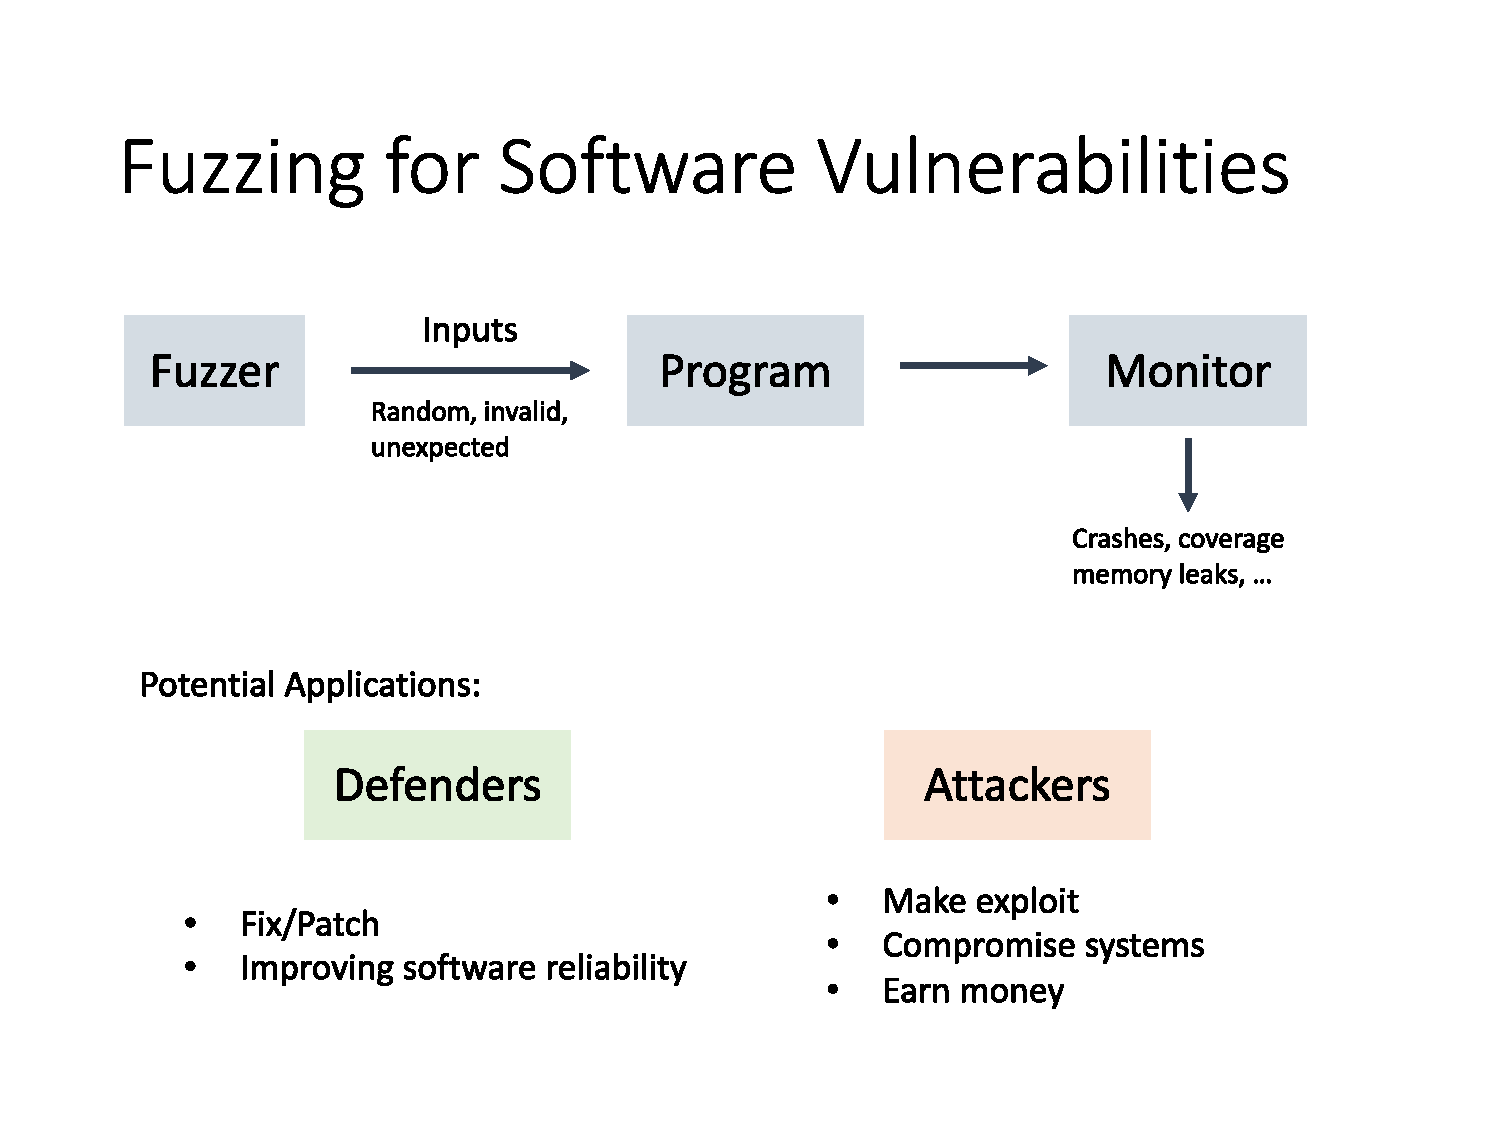
\includegraphics[width=\unitlength,page=1]{Figures/L4_fuzzer_pipeline.pdf}}%
  \end{picture}%
\endgroup%
    
\end{minipage}

\begin{multicols}{2}
 \textbf{Functional Testing}  \\ \rule{\linewidth}{0.4pt} \\ Run programs on \textcolor{green}{well-structured} and \textcolor{green}{normal} inputs (e.g., unit tests) \\ \\ Prevent \textcolor{green}{normal users} from encountering functionality errors  (e.g., assertion failures) 
 \columnbreak 
 \\ \textbf{Fuzzing}  \\ \rule{\linewidth}{0.4pt}  \\ Test programs on \textcolor{red}{abnormal} inputs (e.g., randomly generated \\ \\ Prevent \textcolor{red}{attackers} from making exploits (e.g., memory leaks)
 
\end{multicols}


\paragraph{Fuzzer Categories:}
\begin{description}
    \item \textbf{\textcolor{blue}{Black-Box}} \textbf{No information} about the program or inputs \textcolor{green}{Easy-to-use and fast}, but \textcolor{red}{only explore shallow states}
    \item \textbf{\textcolor{blue}{Grammar-based}} Generate inputs specified a \textbf{grammar}. \textcolor{green}{Can reach deeper states}, but \textcolor{red}{assume a grammar}
    \item \textbf{\textcolor{blue}{White-box}} Use \textbf{heavy-weight program analysis} to generate inputs. \textcolor{green}{Can reach deeper states}, but \textcolor{red}{computationally expensive}
    \item \textbf{\textcolor{blue}{Grey-box}} Use \textbf{light-weight} instrumentation for getting input coverage. \textcolor{green}{Can reach deeper states }, but \textcolor{red}{need careful tuning}
\end{description}{}
\paragraph{Fuzzing Inputs:}
\begin{itemize}
    \item \textbf{\textcolor{blue}{Mutation}} Mutate from "good" seed inputs
        \begin{itemize}
            \item[\color{green}+] Easy to setup
            \item[\color{green}+] No input format specification required
            \item[\color{red}--] Seed inputs required
            \item[\color{red}--] May fail for complex functions (e.g., checksum)
        \end{itemize}
    \item \textbf{\textcolor{blue}{Generation}} Generate inputs from scratch, usually by a grammar
    \begin{itemize} 
        \item[\color{green}+] No need for seed inputs
        \item[\color{red}--] Labor expensive to write generators 
        \item[\color{red}--] Input formed specification required
    \end{itemize}
\end{itemize}
\paragraph{American Fuzzy Loop \textbf{AFL}:}
\begin{itemize}
    \item AFL is a mutational, grey-box fuzzer, with (compile-time or binary-level) instrumentation for branch coverage
    \item Starts a queue from a set of seed inputs
    \item Generates new test cases by mutation from the queue:
    \begin{itemize}
        \item bit or byte flips
        \item addition or subtraction of small integers to bytes
        \item test cases splicing
    \end{itemize}
    \item Add new test case to the queue if new branches are triggered.
\end{itemize}

TODO ILF and Compiler fuzzing examples
\subsection{Symbolic Execution}
\begin{itemize}
\item We associate each variables with a \textcolor{green}{symbolic value} instead of a concrete value.
\item We then run the program with the symbolic values, and obtain a \textcolor{green}{constraint formula}
\item At any program point, we can invoke a constraint (SMT) solver to find \textcolor{green}{satisfying assignments} to the formula, which can be used to indicate \textcolor{green}{concrete inputs} reaching the program point.
\end{itemize}{}

\paragraph{Tracking:}
Symbolic Execution tracks the following two formulas:
\begin{itemize}
    \item \textcolor{green}{symbolic store}: Tracks possible values of variables
    \item \textcolor{green}{path constraint}: Tracks history of all branches taken so far
\end{itemize}{}
\textcolor{green}{Symbolic state} is then defined as the \textcolor{green}{conjunction} of these two formulas
\paragraph{Example:\newline}

\noindent\begin{minipage}{0.5\linewidth}
    \centering      
    \def\svgwidth{\linewidth}
    %% Creator: Inkscape inkscape 0.92.4, www.inkscape.org
%% PDF/EPS/PS + LaTeX output extension by Johan Engelen, 2010
%% Accompanies image file 'L4_symbolic_execution_example_1.pdf' (pdf, eps, ps)
%%
%% To include the image in your LaTeX document, write
%%   \input{<filename>.pdf_tex}
%%  instead of
%%   \includegraphics{<filename>.pdf}
%% To scale the image, write
%%   \def\svgwidth{<desired width>}
%%   \input{<filename>.pdf_tex}
%%  instead of
%%   \includegraphics[width=<desired width>]{<filename>.pdf}
%%
%% Images with a different path to the parent latex file can
%% be accessed with the `import' package (which may need to be
%% installed) using
%%   \usepackage{import}
%% in the preamble, and then including the image with
%%   \import{<path to file>}{<filename>.pdf_tex}
%% Alternatively, one can specify
%%   \graphicspath{{<path to file>/}}
%% 
%% For more information, please see info/svg-inkscape on CTAN:
%%   http://tug.ctan.org/tex-archive/info/svg-inkscape
%%
\begingroup%
  \makeatletter%
  \providecommand\color[2][]{%
    \errmessage{(Inkscape) Color is used for the text in Inkscape, but the package 'color.sty' is not loaded}%
    \renewcommand\color[2][]{}%
  }%
  \providecommand\transparent[1]{%
    \errmessage{(Inkscape) Transparency is used (non-zero) for the text in Inkscape, but the package 'transparent.sty' is not loaded}%
    \renewcommand\transparent[1]{}%
  }%
  \providecommand\rotatebox[2]{#2}%
  \newcommand*\fsize{\dimexpr\f@size pt\relax}%
  \newcommand*\lineheight[1]{\fontsize{\fsize}{#1\fsize}\selectfont}%
  \ifx\svgwidth\undefined%
    \setlength{\unitlength}{596.55861201bp}%
    \ifx\svgscale\undefined%
      \relax%
    \else%
      \setlength{\unitlength}{\unitlength * \real{\svgscale}}%
    \fi%
  \else%
    \setlength{\unitlength}{\svgwidth}%
  \fi%
  \global\let\svgwidth\undefined%
  \global\let\svgscale\undefined%
  \makeatother%
  \begin{picture}(1,0.61038899)%
    \lineheight{1}%
    \setlength\tabcolsep{0pt}%
    \put(0,0){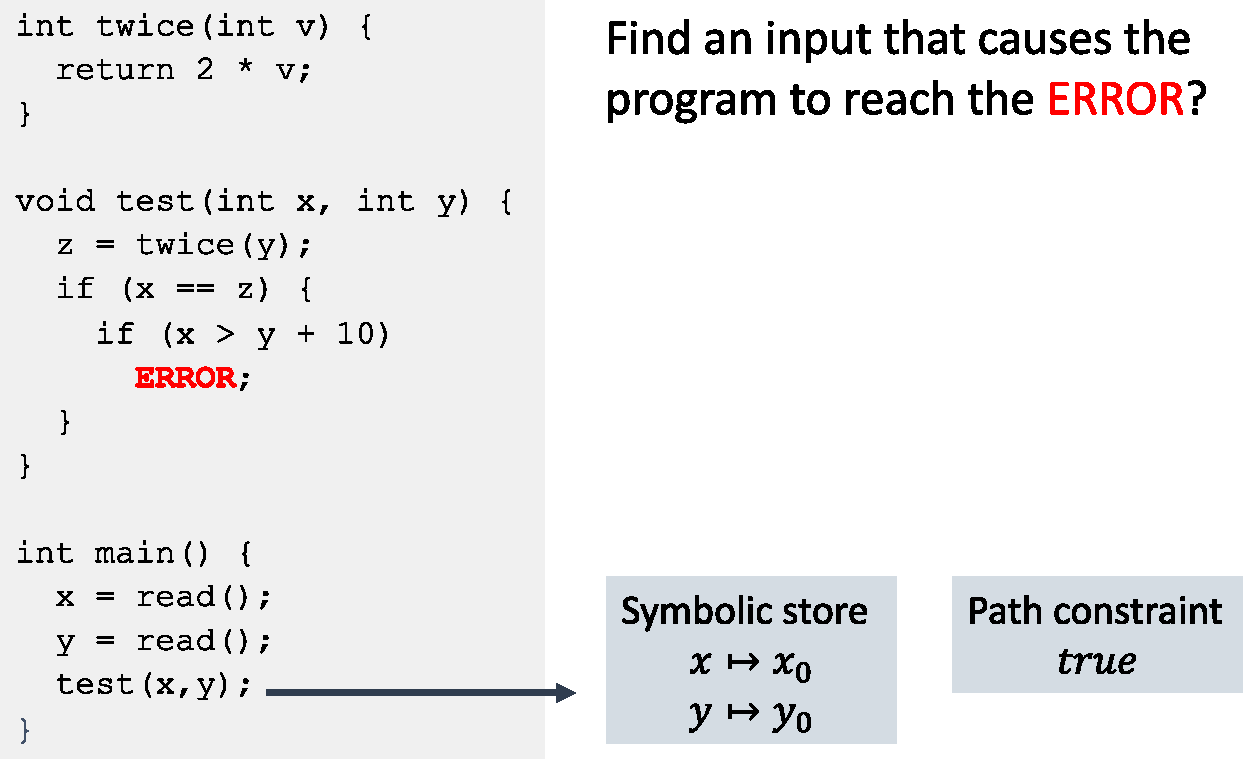
\includegraphics[width=\unitlength,page=1]{Figures/L4_symbolic_execution_example_1.pdf}}%
  \end{picture}%
\endgroup%
    
\end{minipage}
\begin{minipage}{0.5\linewidth}
    \centering      
    \def\svgwidth{\linewidth}
    %% Creator: Inkscape inkscape 0.92.4, www.inkscape.org
%% PDF/EPS/PS + LaTeX output extension by Johan Engelen, 2010
%% Accompanies image file 'L4_symbolic_execution_example_2.pdf' (pdf, eps, ps)
%%
%% To include the image in your LaTeX document, write
%%   \input{<filename>.pdf_tex}
%%  instead of
%%   \includegraphics{<filename>.pdf}
%% To scale the image, write
%%   \def\svgwidth{<desired width>}
%%   \input{<filename>.pdf_tex}
%%  instead of
%%   \includegraphics[width=<desired width>]{<filename>.pdf}
%%
%% Images with a different path to the parent latex file can
%% be accessed with the `import' package (which may need to be
%% installed) using
%%   \usepackage{import}
%% in the preamble, and then including the image with
%%   \import{<path to file>}{<filename>.pdf_tex}
%% Alternatively, one can specify
%%   \graphicspath{{<path to file>/}}
%% 
%% For more information, please see info/svg-inkscape on CTAN:
%%   http://tug.ctan.org/tex-archive/info/svg-inkscape
%%
\begingroup%
  \makeatletter%
  \providecommand\color[2][]{%
    \errmessage{(Inkscape) Color is used for the text in Inkscape, but the package 'color.sty' is not loaded}%
    \renewcommand\color[2][]{}%
  }%
  \providecommand\transparent[1]{%
    \errmessage{(Inkscape) Transparency is used (non-zero) for the text in Inkscape, but the package 'transparent.sty' is not loaded}%
    \renewcommand\transparent[1]{}%
  }%
  \providecommand\rotatebox[2]{#2}%
  \newcommand*\fsize{\dimexpr\f@size pt\relax}%
  \newcommand*\lineheight[1]{\fontsize{\fsize}{#1\fsize}\selectfont}%
  \ifx\svgwidth\undefined%
    \setlength{\unitlength}{610.37889375bp}%
    \ifx\svgscale\undefined%
      \relax%
    \else%
      \setlength{\unitlength}{\unitlength * \real{\svgscale}}%
    \fi%
  \else%
    \setlength{\unitlength}{\svgwidth}%
  \fi%
  \global\let\svgwidth\undefined%
  \global\let\svgscale\undefined%
  \makeatother%
  \begin{picture}(1,0.59656847)%
    \lineheight{1}%
    \setlength\tabcolsep{0pt}%
    \put(0,0){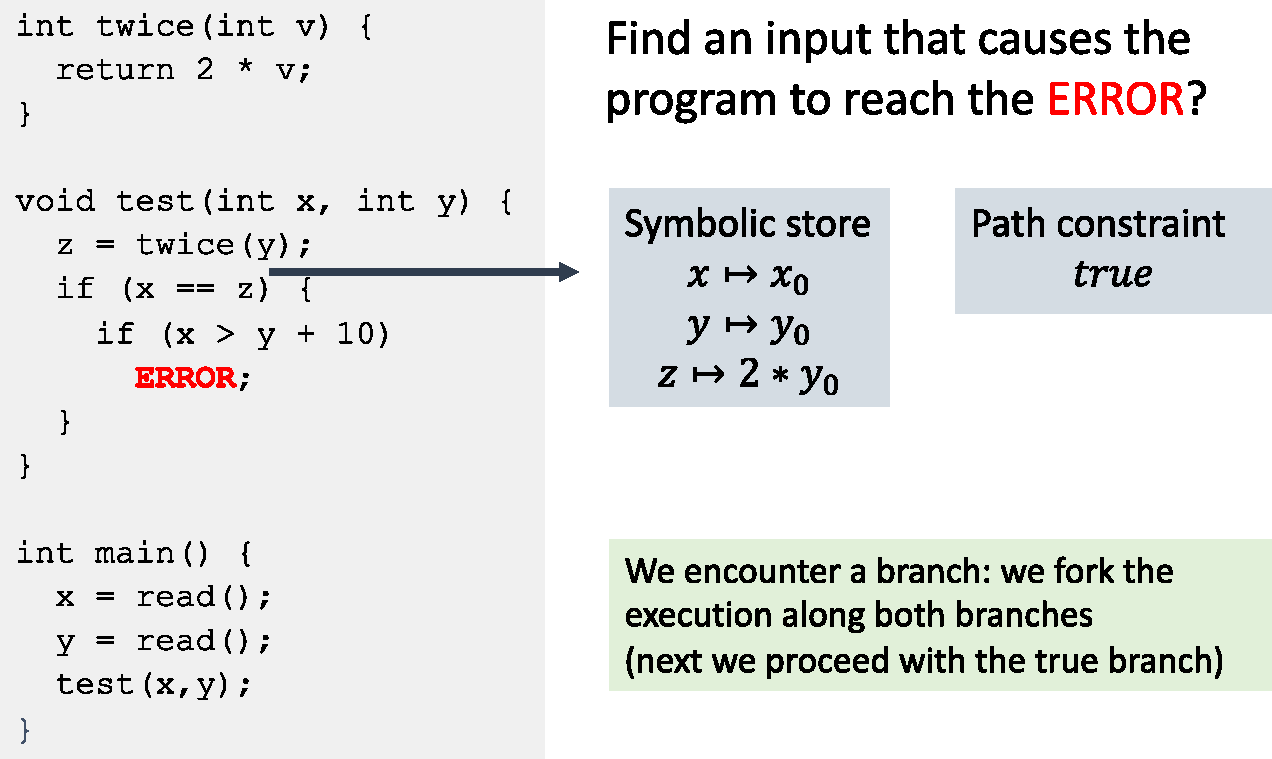
\includegraphics[width=\unitlength,page=1]{Figures/L4_symbolic_execution_example_2.pdf}}%
  \end{picture}%
\endgroup%
    
\end{minipage}
\begin{minipage}{0.5\linewidth}
    \centering      
    \def\svgwidth{\linewidth}
    %% Creator: Inkscape inkscape 0.92.4, www.inkscape.org
%% PDF/EPS/PS + LaTeX output extension by Johan Engelen, 2010
%% Accompanies image file 'L4_symbolic_execution_example.pdf' (pdf, eps, ps)
%%
%% To include the image in your LaTeX document, write
%%   \input{<filename>.pdf_tex}
%%  instead of
%%   \includegraphics{<filename>.pdf}
%% To scale the image, write
%%   \def\svgwidth{<desired width>}
%%   \input{<filename>.pdf_tex}
%%  instead of
%%   \includegraphics[width=<desired width>]{<filename>.pdf}
%%
%% Images with a different path to the parent latex file can
%% be accessed with the `import' package (which may need to be
%% installed) using
%%   \usepackage{import}
%% in the preamble, and then including the image with
%%   \import{<path to file>}{<filename>.pdf_tex}
%% Alternatively, one can specify
%%   \graphicspath{{<path to file>/}}
%% 
%% For more information, please see info/svg-inkscape on CTAN:
%%   http://tug.ctan.org/tex-archive/info/svg-inkscape
%%
\begingroup%
  \makeatletter%
  \providecommand\color[2][]{%
    \errmessage{(Inkscape) Color is used for the text in Inkscape, but the package 'color.sty' is not loaded}%
    \renewcommand\color[2][]{}%
  }%
  \providecommand\transparent[1]{%
    \errmessage{(Inkscape) Transparency is used (non-zero) for the text in Inkscape, but the package 'transparent.sty' is not loaded}%
    \renewcommand\transparent[1]{}%
  }%
  \providecommand\rotatebox[2]{#2}%
  \newcommand*\fsize{\dimexpr\f@size pt\relax}%
  \newcommand*\lineheight[1]{\fontsize{\fsize}{#1\fsize}\selectfont}%
  \ifx\svgwidth\undefined%
    \setlength{\unitlength}{608.67968942bp}%
    \ifx\svgscale\undefined%
      \relax%
    \else%
      \setlength{\unitlength}{\unitlength * \real{\svgscale}}%
    \fi%
  \else%
    \setlength{\unitlength}{\svgwidth}%
  \fi%
  \global\let\svgwidth\undefined%
  \global\let\svgscale\undefined%
  \makeatother%
  \begin{picture}(1,0.59823387)%
    \lineheight{1}%
    \setlength\tabcolsep{0pt}%
    \put(0,0){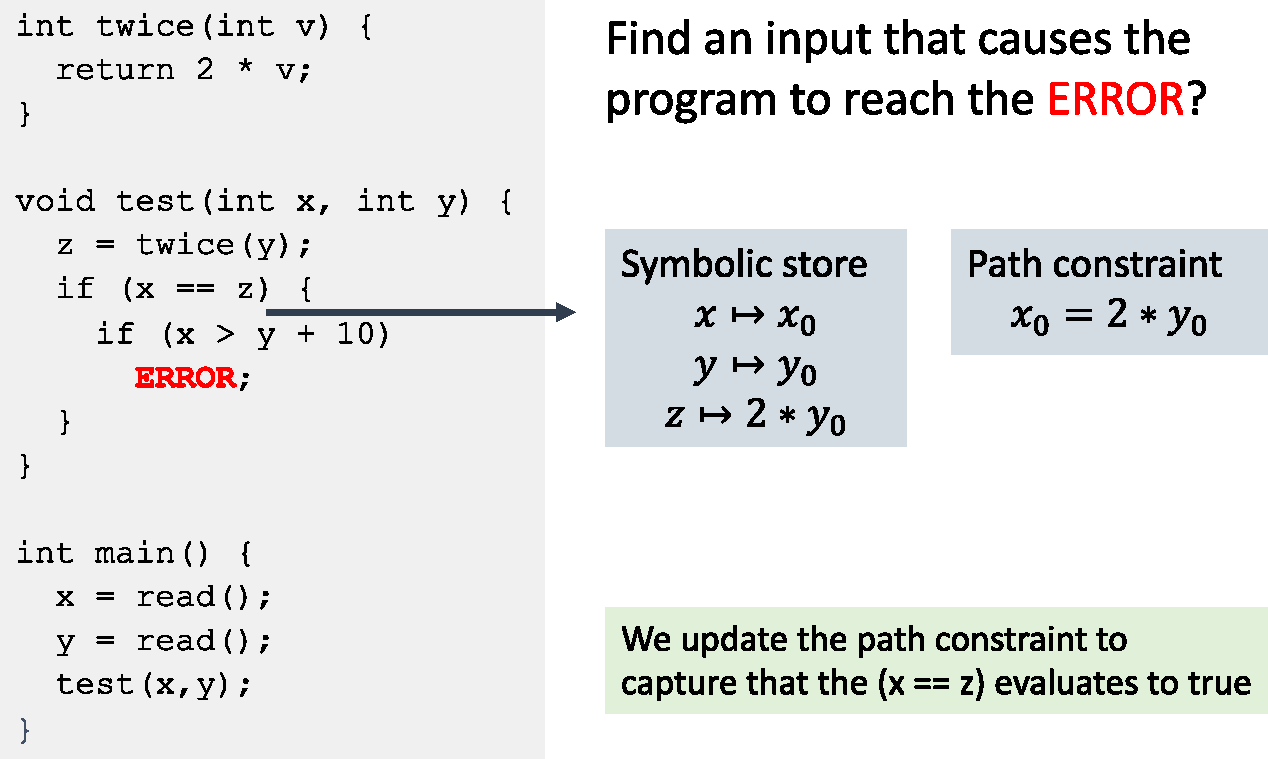
\includegraphics[width=\unitlength,page=1]{Figures/L4_symbolic_execution_example_3.pdf}}%
  \end{picture}%
\endgroup%
    
\end{minipage}
\begin{minipage}{0.5\linewidth}
    \centering      
    \def\svgwidth{\linewidth}
    %% Creator: Inkscape inkscape 0.92.4, www.inkscape.org
%% PDF/EPS/PS + LaTeX output extension by Johan Engelen, 2010
%% Accompanies image file 'L4_symbolic_execution_example_2.pdf' (pdf, eps, ps)
%%
%% To include the image in your LaTeX document, write
%%   \input{<filename>.pdf_tex}
%%  instead of
%%   \includegraphics{<filename>.pdf}
%% To scale the image, write
%%   \def\svgwidth{<desired width>}
%%   \input{<filename>.pdf_tex}
%%  instead of
%%   \includegraphics[width=<desired width>]{<filename>.pdf}
%%
%% Images with a different path to the parent latex file can
%% be accessed with the `import' package (which may need to be
%% installed) using
%%   \usepackage{import}
%% in the preamble, and then including the image with
%%   \import{<path to file>}{<filename>.pdf_tex}
%% Alternatively, one can specify
%%   \graphicspath{{<path to file>/}}
%% 
%% For more information, please see info/svg-inkscape on CTAN:
%%   http://tug.ctan.org/tex-archive/info/svg-inkscape
%%
\begingroup%
  \makeatletter%
  \providecommand\color[2][]{%
    \errmessage{(Inkscape) Color is used for the text in Inkscape, but the package 'color.sty' is not loaded}%
    \renewcommand\color[2][]{}%
  }%
  \providecommand\transparent[1]{%
    \errmessage{(Inkscape) Transparency is used (non-zero) for the text in Inkscape, but the package 'transparent.sty' is not loaded}%
    \renewcommand\transparent[1]{}%
  }%
  \providecommand\rotatebox[2]{#2}%
  \newcommand*\fsize{\dimexpr\f@size pt\relax}%
  \newcommand*\lineheight[1]{\fontsize{\fsize}{#1\fsize}\selectfont}%
  \ifx\svgwidth\undefined%
    \setlength{\unitlength}{638.22863001bp}%
    \ifx\svgscale\undefined%
      \relax%
    \else%
      \setlength{\unitlength}{\unitlength * \real{\svgscale}}%
    \fi%
  \else%
    \setlength{\unitlength}{\svgwidth}%
  \fi%
  \global\let\svgwidth\undefined%
  \global\let\svgscale\undefined%
  \makeatother%
  \begin{picture}(1,0.57336693)%
    \lineheight{1}%
    \setlength\tabcolsep{0pt}%
    \put(0,0){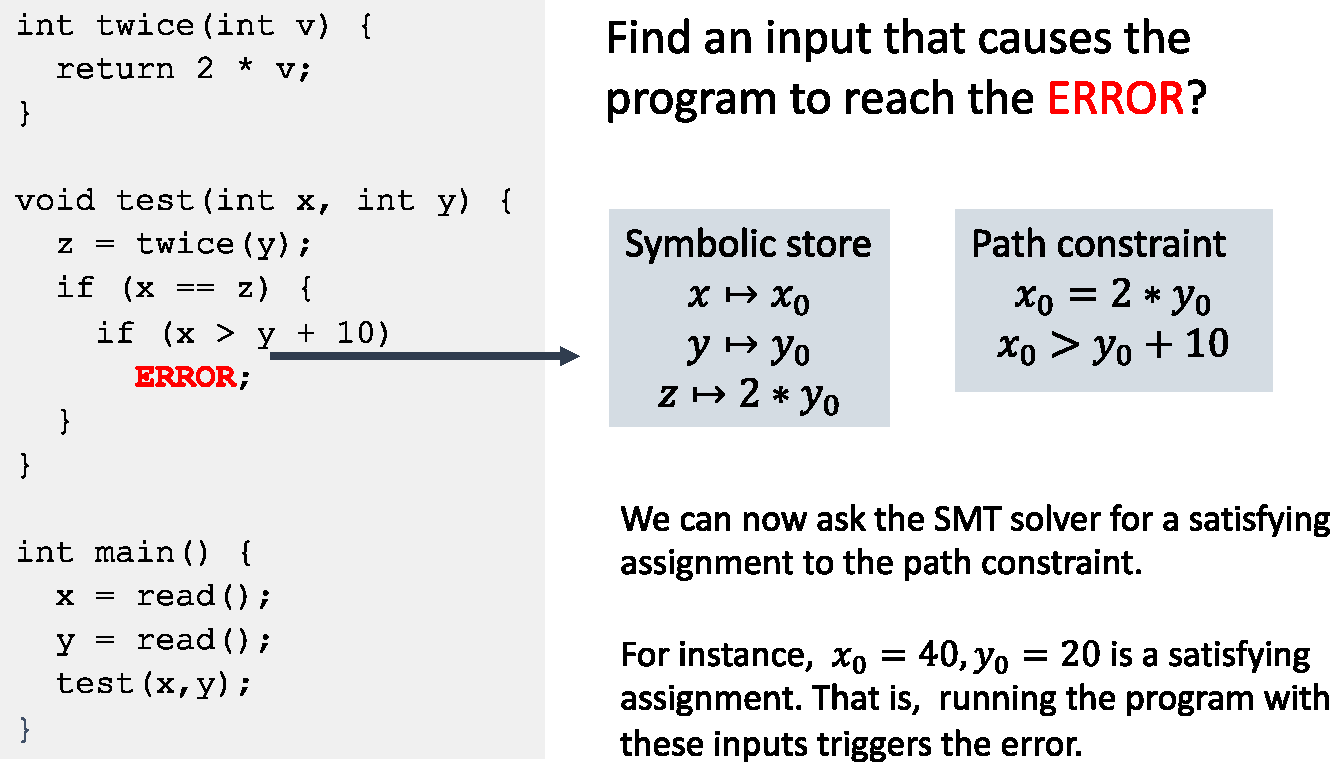
\includegraphics[width=\unitlength,page=1]{Figures/L4_symbolic_execution_example_4.pdf}}%
  \end{picture}%
\endgroup%
    
\end{minipage}

\paragraph{In Practice:}
\begin{itemize}
\item Many challenges:
\begin{itemize}
    \item Path explosion (exponential in number of branches)
    \item Constraint solving (e.g., non-linear and hash constraints)
\end{itemize}{}
\item Real-world symbolic execution fuzzers:
\begin{itemize}
    \item Stanford KLEE (http://klee.github.io/)
    \item NASA’s Java PathFinder (http://javapathfinder.sourceforge.net/)
    \item Microsoft SAGE
    \item UC Berkeley’s CUTE
\end{itemize}{}
\end{itemize}{}

\paragraph{Comparison:}
\begin{minipage}{0.5\linewidth}
    \centering      
    \def\svgwidth{\linewidth}
    %% Creator: Inkscape inkscape 0.92.4, www.inkscape.org
%% PDF/EPS/PS + LaTeX output extension by Johan Engelen, 2010
%% Accompanies image file 'L4_symbolic_execution_vs_Fuzzing.pdf' (pdf, eps, ps)
%%
%% To include the image in your LaTeX document, write
%%   \input{<filename>.pdf_tex}
%%  instead of
%%   \includegraphics{<filename>.pdf}
%% To scale the image, write
%%   \def\svgwidth{<desired width>}
%%   \input{<filename>.pdf_tex}
%%  instead of
%%   \includegraphics[width=<desired width>]{<filename>.pdf}
%%
%% Images with a different path to the parent latex file can
%% be accessed with the `import' package (which may need to be
%% installed) using
%%   \usepackage{import}
%% in the preamble, and then including the image with
%%   \import{<path to file>}{<filename>.pdf_tex}
%% Alternatively, one can specify
%%   \graphicspath{{<path to file>/}}
%% 
%% For more information, please see info/svg-inkscape on CTAN:
%%   http://tug.ctan.org/tex-archive/info/svg-inkscape
%%
\begingroup%
  \makeatletter%
  \providecommand\color[2][]{%
    \errmessage{(Inkscape) Color is used for the text in Inkscape, but the package 'color.sty' is not loaded}%
    \renewcommand\color[2][]{}%
  }%
  \providecommand\transparent[1]{%
    \errmessage{(Inkscape) Transparency is used (non-zero) for the text in Inkscape, but the package 'transparent.sty' is not loaded}%
    \renewcommand\transparent[1]{}%
  }%
  \providecommand\rotatebox[2]{#2}%
  \newcommand*\fsize{\dimexpr\f@size pt\relax}%
  \newcommand*\lineheight[1]{\fontsize{\fsize}{#1\fsize}\selectfont}%
  \ifx\svgwidth\undefined%
    \setlength{\unitlength}{578.74250757bp}%
    \ifx\svgscale\undefined%
      \relax%
    \else%
      \setlength{\unitlength}{\unitlength * \real{\svgscale}}%
    \fi%
  \else%
    \setlength{\unitlength}{\svgwidth}%
  \fi%
  \global\let\svgwidth\undefined%
  \global\let\svgscale\undefined%
  \makeatother%
  \begin{picture}(1,0.44964702)%
    \lineheight{1}%
    \setlength\tabcolsep{0pt}%
    \put(0,0){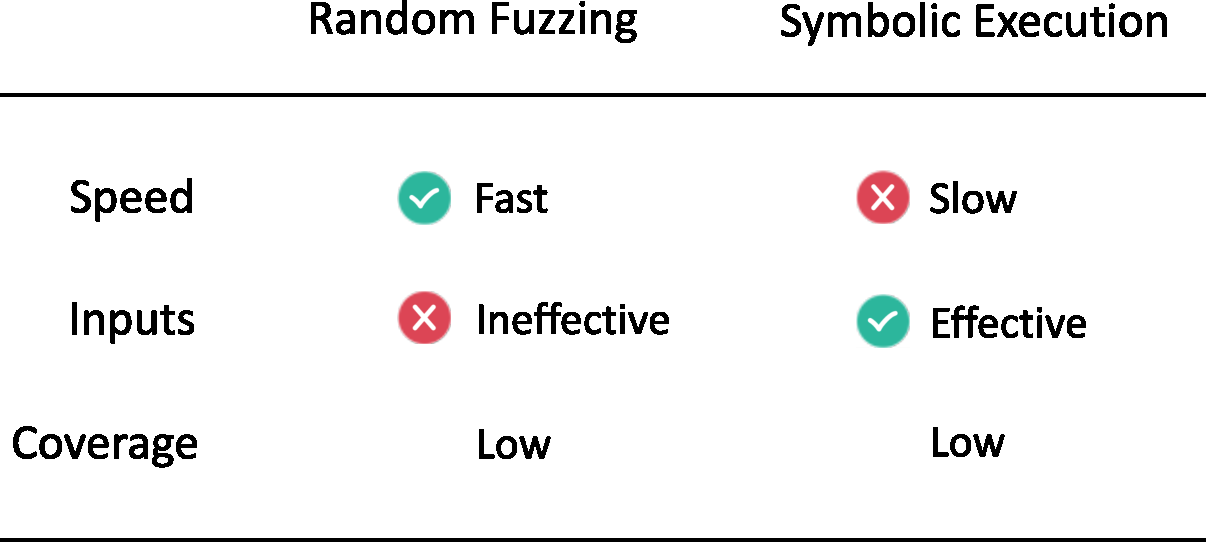
\includegraphics[width=\unitlength,page=1]{Figures/L4_symbolic_execution_vs_Fuzzing.pdf}}%
  \end{picture}%
\endgroup%
    
\end{minipage}

\subsection{Imitation Learning based Fuzzer ILF}

\begin{minipage}{0.75\linewidth}
    \centering      
    \def\svgwidth{\linewidth}
    %% Creator: Inkscape inkscape 0.92.4, www.inkscape.org
%% PDF/EPS/PS + LaTeX output extension by Johan Engelen, 2010
%% Accompanies image file 'L4_ILF.pdf' (pdf, eps, ps)
%%
%% To include the image in your LaTeX document, write
%%   \input{<filename>.pdf_tex}
%%  instead of
%%   \includegraphics{<filename>.pdf}
%% To scale the image, write
%%   \def\svgwidth{<desired width>}
%%   \input{<filename>.pdf_tex}
%%  instead of
%%   \includegraphics[width=<desired width>]{<filename>.pdf}
%%
%% Images with a different path to the parent latex file can
%% be accessed with the `import' package (which may need to be
%% installed) using
%%   \usepackage{import}
%% in the preamble, and then including the image with
%%   \import{<path to file>}{<filename>.pdf_tex}
%% Alternatively, one can specify
%%   \graphicspath{{<path to file>/}}
%% 
%% For more information, please see info/svg-inkscape on CTAN:
%%   http://tug.ctan.org/tex-archive/info/svg-inkscape
%%
\begingroup%
  \makeatletter%
  \providecommand\color[2][]{%
    \errmessage{(Inkscape) Color is used for the text in Inkscape, but the package 'color.sty' is not loaded}%
    \renewcommand\color[2][]{}%
  }%
  \providecommand\transparent[1]{%
    \errmessage{(Inkscape) Transparency is used (non-zero) for the text in Inkscape, but the package 'transparent.sty' is not loaded}%
    \renewcommand\transparent[1]{}%
  }%
  \providecommand\rotatebox[2]{#2}%
  \newcommand*\fsize{\dimexpr\f@size pt\relax}%
  \newcommand*\lineheight[1]{\fontsize{\fsize}{#1\fsize}\selectfont}%
  \ifx\svgwidth\undefined%
    \setlength{\unitlength}{634.3925416bp}%
    \ifx\svgscale\undefined%
      \relax%
    \else%
      \setlength{\unitlength}{\unitlength * \real{\svgscale}}%
    \fi%
  \else%
    \setlength{\unitlength}{\svgwidth}%
  \fi%
  \global\let\svgwidth\undefined%
  \global\let\svgscale\undefined%
  \makeatother%
  \begin{picture}(1,0.49303044)%
    \lineheight{1}%
    \setlength\tabcolsep{0pt}%
    \put(0,0){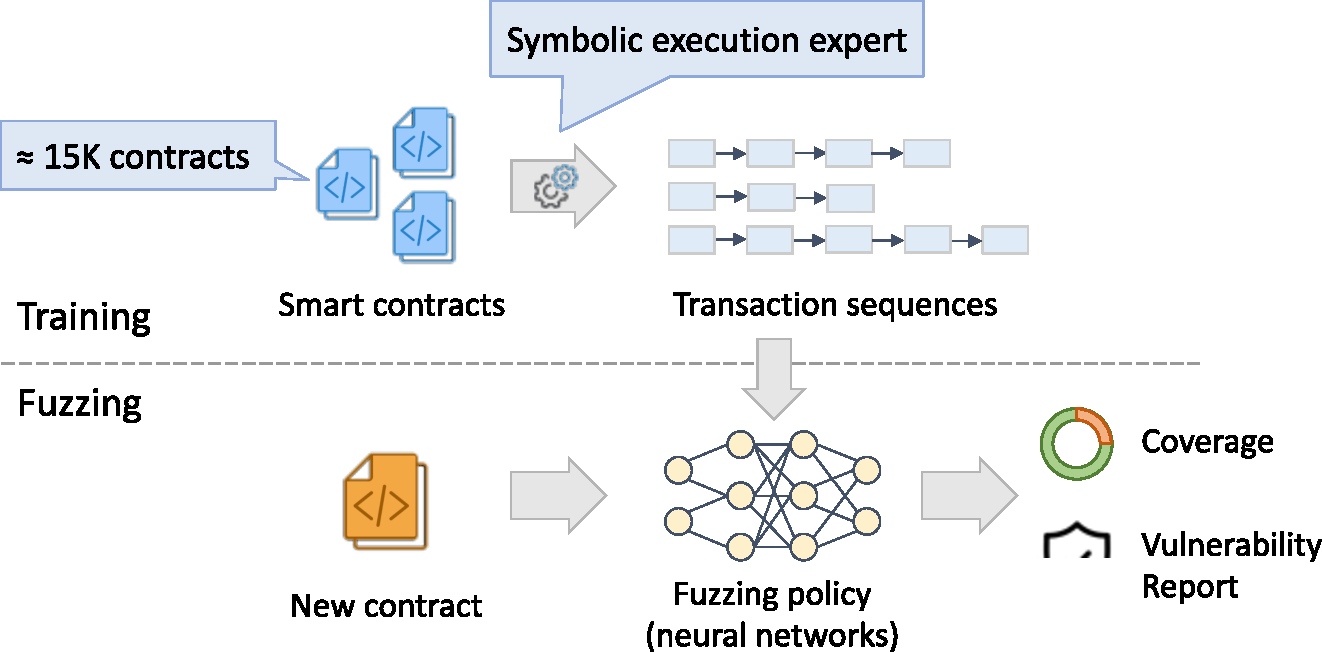
\includegraphics[width=\unitlength,page=1]{Figures/L4_ILF.pdf}}%
  \end{picture}%
\endgroup%
    
\end{minipage}
\paragraph{Fuzzing Policy:\newline}
\begin{minipage}{0.5\linewidth}
    \centering      
    \def\svgwidth{\linewidth}
    %% Creator: Inkscape inkscape 0.92.4, www.inkscape.org
%% PDF/EPS/PS + LaTeX output extension by Johan Engelen, 2010
%% Accompanies image file 'L4_ILF_fuzzing_policy.pdf' (pdf, eps, ps)
%%
%% To include the image in your LaTeX document, write
%%   \input{<filename>.pdf_tex}
%%  instead of
%%   \includegraphics{<filename>.pdf}
%% To scale the image, write
%%   \def\svgwidth{<desired width>}
%%   \input{<filename>.pdf_tex}
%%  instead of
%%   \includegraphics[width=<desired width>]{<filename>.pdf}
%%
%% Images with a different path to the parent latex file can
%% be accessed with the `import' package (which may need to be
%% installed) using
%%   \usepackage{import}
%% in the preamble, and then including the image with
%%   \import{<path to file>}{<filename>.pdf_tex}
%% Alternatively, one can specify
%%   \graphicspath{{<path to file>/}}
%% 
%% For more information, please see info/svg-inkscape on CTAN:
%%   http://tug.ctan.org/tex-archive/info/svg-inkscape
%%
\begingroup%
  \makeatletter%
  \providecommand\color[2][]{%
    \errmessage{(Inkscape) Color is used for the text in Inkscape, but the package 'color.sty' is not loaded}%
    \renewcommand\color[2][]{}%
  }%
  \providecommand\transparent[1]{%
    \errmessage{(Inkscape) Transparency is used (non-zero) for the text in Inkscape, but the package 'transparent.sty' is not loaded}%
    \renewcommand\transparent[1]{}%
  }%
  \providecommand\rotatebox[2]{#2}%
  \newcommand*\fsize{\dimexpr\f@size pt\relax}%
  \newcommand*\lineheight[1]{\fontsize{\fsize}{#1\fsize}\selectfont}%
  \ifx\svgwidth\undefined%
    \setlength{\unitlength}{651.1706543bp}%
    \ifx\svgscale\undefined%
      \relax%
    \else%
      \setlength{\unitlength}{\unitlength * \real{\svgscale}}%
    \fi%
  \else%
    \setlength{\unitlength}{\svgwidth}%
  \fi%
  \global\let\svgwidth\undefined%
  \global\let\svgscale\undefined%
  \makeatother%
  \begin{picture}(1,0.5471154)%
    \lineheight{1}%
    \setlength\tabcolsep{0pt}%
    \put(0,0){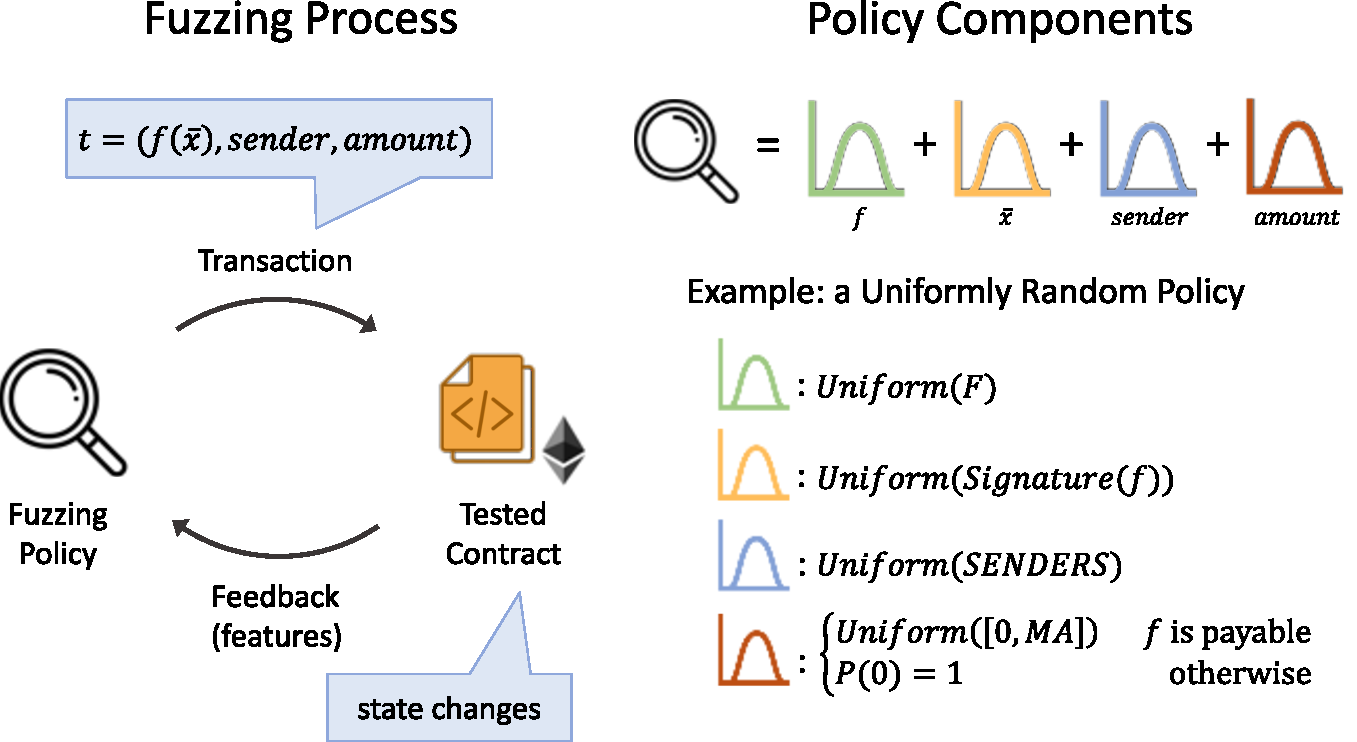
\includegraphics[width=\unitlength,page=1]{Figures/L4_ILF_fuzzing_policy.pdf}}%
  \end{picture}%
\endgroup%
    
\end{minipage}
\begin{minipage}{0.5\linewidth}
    \centering      
    \def\svgwidth{\linewidth}
    %% Creator: Inkscape inkscape 0.92.4, www.inkscape.org
%% PDF/EPS/PS + LaTeX output extension by Johan Engelen, 2010
%% Accompanies image file 'L4_ILF_fuzzing_policy.pdf' (pdf, eps, ps)
%%
%% To include the image in your LaTeX document, write
%%   \input{<filename>.pdf_tex}
%%  instead of
%%   \includegraphics{<filename>.pdf}
%% To scale the image, write
%%   \def\svgwidth{<desired width>}
%%   \input{<filename>.pdf_tex}
%%  instead of
%%   \includegraphics[width=<desired width>]{<filename>.pdf}
%%
%% Images with a different path to the parent latex file can
%% be accessed with the `import' package (which may need to be
%% installed) using
%%   \usepackage{import}
%% in the preamble, and then including the image with
%%   \import{<path to file>}{<filename>.pdf_tex}
%% Alternatively, one can specify
%%   \graphicspath{{<path to file>/}}
%% 
%% For more information, please see info/svg-inkscape on CTAN:
%%   http://tug.ctan.org/tex-archive/info/svg-inkscape
%%
\begingroup%
  \makeatletter%
  \providecommand\color[2][]{%
    \errmessage{(Inkscape) Color is used for the text in Inkscape, but the package 'color.sty' is not loaded}%
    \renewcommand\color[2][]{}%
  }%
  \providecommand\transparent[1]{%
    \errmessage{(Inkscape) Transparency is used (non-zero) for the text in Inkscape, but the package 'transparent.sty' is not loaded}%
    \renewcommand\transparent[1]{}%
  }%
  \providecommand\rotatebox[2]{#2}%
  \newcommand*\fsize{\dimexpr\f@size pt\relax}%
  \newcommand*\lineheight[1]{\fontsize{\fsize}{#1\fsize}\selectfont}%
  \ifx\svgwidth\undefined%
    \setlength{\unitlength}{634.74825641bp}%
    \ifx\svgscale\undefined%
      \relax%
    \else%
      \setlength{\unitlength}{\unitlength * \real{\svgscale}}%
    \fi%
  \else%
    \setlength{\unitlength}{\svgwidth}%
  \fi%
  \global\let\svgwidth\undefined%
  \global\let\svgscale\undefined%
  \makeatother%
  \begin{picture}(1,0.45047456)%
    \lineheight{1}%
    \setlength\tabcolsep{0pt}%
    \put(0,0){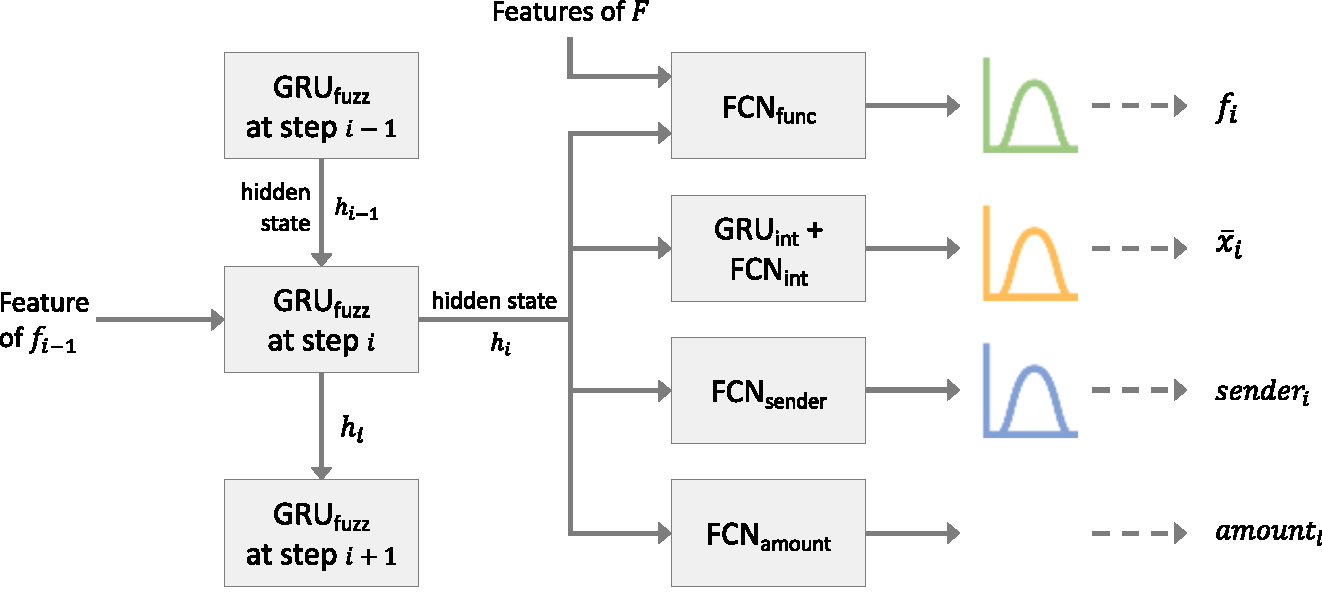
\includegraphics[width=\unitlength,page=1]{Figures/L4_ILF_fuzzing_policy_detail.pdf}}%
  \end{picture}%
\endgroup%
    
\end{minipage}
\begin{itemize}
    \item \textbf{GRU}: Gated Recurrent Units
    \begin{itemize}
        \item Can deal with variable length \textcolor{green}{sequential} inputs with hidden states
        \item A natural fit for our setting for handling \textcolor{green}{sequence of transactions}
    \end{itemize}{}
    \item Features of $f_{i-1}$ could be Coverage, opcodes, function name. (can be dynamic)
    \item Fully Connected Networks (\textbf{FCN}): Standard network with linear layers and ReLU activation functions
    \item Softmax: Normalizes function scores (output of \textbf{FCN$_{func}$}) to probability distrubtion
\end{itemize}{}
\textbf{Neural Network description}:

\begin{itemize}
    \item \textbf{Function: } FCN$_{func}$ + Softmax
    \item \textbf{Arguments: } GRU$_{int}$ + FCN$_{int}$. Initial distribution from expert. Challenges:
        \begin{itemize}
            \item Functions have a \textcolor{red}{variable} length of arguments
            \item Search space of arguments is \textcolor{red}{large} (e.g., integers of 256 bits)
        \end{itemize}{}
     \item \textbf{Senders: }  FCN$_{sender}$. Distribution over 5 predefined senders
      \item \textbf{Amount: }  FCN$_{amount}$. Distribution over 50 seed amount values from expert
\end{itemize}{}
\paragraph{Symbolic Execution Expert:}
\begin{itemize}
    \item Standard symbolic engines (breadth-first style):
    \begin{itemize}
        \item Operate on symbolic blockchain state and generate symbolictransactions.
        \item Only scale to limited depth (e.g. 3)
    \end{itemize}{}
    \item Our expert (depth-first style with revisits):
    \begin{itemize}
        \item Operates on concrete blockchain state and generate concrete transactions.
        \item Scales to large depth (e.g. 30) and large training set.
        \item Algorithm:
        \begin{enumerate}
            \item Start on initial blockchain state $b_{init}$
            \item Greedy search for transaction $t$ with highest coverage
            \item Execute transaction $t$ to get to next blockchain state $b_1$
            \item Revisit blockchain states $b_i$ and take different transactions to improve code coverage
            \item Repeat
        \end{enumerate}{}
 \end{itemize}
\end{itemize}{}
\paragraph{Miscellaneous}
\begin{itemize}
    \item \textbf{Training NN Fuzzing Policy: } Use Cross-Entropy Loss on inferred transactions and transactions by expert. aka standard supervised learning
    \item \textbf{ILF System: Reports the following:}
    \begin{itemize}
        \item Instruction coverage.
        \item Basic block coverage.
        \item Locking: The contract cannot send out but can receive ether.
        \item Leaking: An attacker can steal ether from the contract.
        \item Suicidal: An attacker can deconstruct the contract.
        \item Block Dependency: Ether transfer depends on block state variables.
        \item Unhandled Exception: Root call does not catch exceptions from child calls.
        \item Controlled Delegatecall: Transaction parameters explicitly flow into arguments of a delegatecall instruction.
    \end{itemize}{}
\end{itemize}{}